\documentclass[1p]{elsarticle_modified}
%\bibliographystyle{elsarticle-num}

%\usepackage[colorlinks]{hyperref}
%\usepackage{abbrmath_seonhwa} %\Abb, \Ascr, \Acal ,\Abf, \Afrak
\usepackage{amsfonts}
\usepackage{amssymb}
\usepackage{amsmath}
\usepackage{amsthm}
\usepackage{scalefnt}
\usepackage{amsbsy}
\usepackage{kotex}
\usepackage{caption}
\usepackage{subfig}
\usepackage{color}
\usepackage{graphicx}
\usepackage{xcolor} %% white, black, red, green, blue, cyan, magenta, yellow
\usepackage{float}
\usepackage{setspace}
\usepackage{hyperref}

\usepackage{tikz}
\usetikzlibrary{arrows}

\usepackage{multirow}
\usepackage{array} % fixed length table
\usepackage{hhline}

%%%%%%%%%%%%%%%%%%%%%
\makeatletter
\renewcommand*\env@matrix[1][\arraystretch]{%
	\edef\arraystretch{#1}%
	\hskip -\arraycolsep
	\let\@ifnextchar\new@ifnextchar
	\array{*\c@MaxMatrixCols c}}
\makeatother %https://tex.stackexchange.com/questions/14071/how-can-i-increase-the-line-spacing-in-a-matrix
%%%%%%%%%%%%%%%

\usepackage[normalem]{ulem}

\newcommand{\msout}[1]{\ifmmode\text{\sout{\ensuremath{#1}}}\else\sout{#1}\fi}
%SOURCE: \msout is \stkout macro in https://tex.stackexchange.com/questions/20609/strikeout-in-math-mode

\newcommand{\cancel}[1]{
	\ifmmode
	{\color{red}\msout{#1}}
	\else
	{\color{red}\sout{#1}}
	\fi
}

\newcommand{\add}[1]{
	{\color{blue}\uwave{#1}}
}

\newcommand{\replace}[2]{
	\ifmmode
	{\color{red}\msout{#1}}{\color{blue}\uwave{#2}}
	\else
	{\color{red}\sout{#1}}{\color{blue}\uwave{#2}}
	\fi
}

\newcommand{\Sol}{\mathcal{S}} %segment
\newcommand{\D}{D} %diagram
\newcommand{\A}{\mathcal{A}} %arc


%%%%%%%%%%%%%%%%%%%%%%%%%%%%%5 test

\def\sl{\operatorname{\textup{SL}}(2,\Cbb)}
\def\psl{\operatorname{\textup{PSL}}(2,\Cbb)}
\def\quan{\mkern 1mu \triangleright \mkern 1mu}

\theoremstyle{definition}
\newtheorem{thm}{Theorem}[section]
\newtheorem{prop}[thm]{Proposition}
\newtheorem{lem}[thm]{Lemma}
\newtheorem{ques}[thm]{Question}
\newtheorem{cor}[thm]{Corollary}
\newtheorem{defn}[thm]{Definition}
\newtheorem{exam}[thm]{Example}
\newtheorem{rmk}[thm]{Remark}
\newtheorem{alg}[thm]{Algorithm}

\newcommand{\I}{\sqrt{-1}}
\begin{document}

%\begin{frontmatter}
%
%\title{Boundary parabolic representations of knots up to 8 crossings}
%
%%% Group authors per affiliation:
%\author{Yunhi Cho} 
%\address{Department of Mathematics, University of Seoul, Seoul, Korea}
%\ead{yhcho@uos.ac.kr}
%
%
%\author{Seonhwa Kim} %\fnref{s_kim}}
%\address{Center for Geometry and Physics, Institute for Basic Science, Pohang, 37673, Korea}
%\ead{ryeona17@ibs.re.kr}
%
%\author{Hyuk Kim}
%\address{Department of Mathematical Sciences, Seoul National University, Seoul 08826, Korea}
%\ead{hyukkim@snu.ac.kr}
%
%\author{Seokbeom Yoon}
%\address{Department of Mathematical Sciences, Seoul National University, Seoul, 08826,  Korea}
%\ead{sbyoon15@snu.ac.kr}
%
%\begin{abstract}
%We find all boundary parabolic representation of knots up to 8 crossings.
%
%\end{abstract}
%\begin{keyword}
%    \MSC[2010] 57M25 
%\end{keyword}
%
%\end{frontmatter}

%\linenumbers
%\tableofcontents
%
\newcommand\colored[1]{\textcolor{white}{\rule[-0.35ex]{0.8em}{1.4ex}}\kern-0.8em\color{red} #1}%
%\newcommand\colored[1]{\textcolor{white}{ #1}\kern-2.17ex	\textcolor{white}{ #1}\kern-1.81ex	\textcolor{white}{ #1}\kern-2.15ex\color{red}#1	}

{\Large $\underline{12n_{0225}~(K12n_{0225})}$}

\setlength{\tabcolsep}{10pt}
\renewcommand{\arraystretch}{1.6}
\vspace{1cm}\begin{tabular}{m{100pt}>{\centering\arraybackslash}m{274pt}}
\multirow{5}{120pt}{
	\centering
	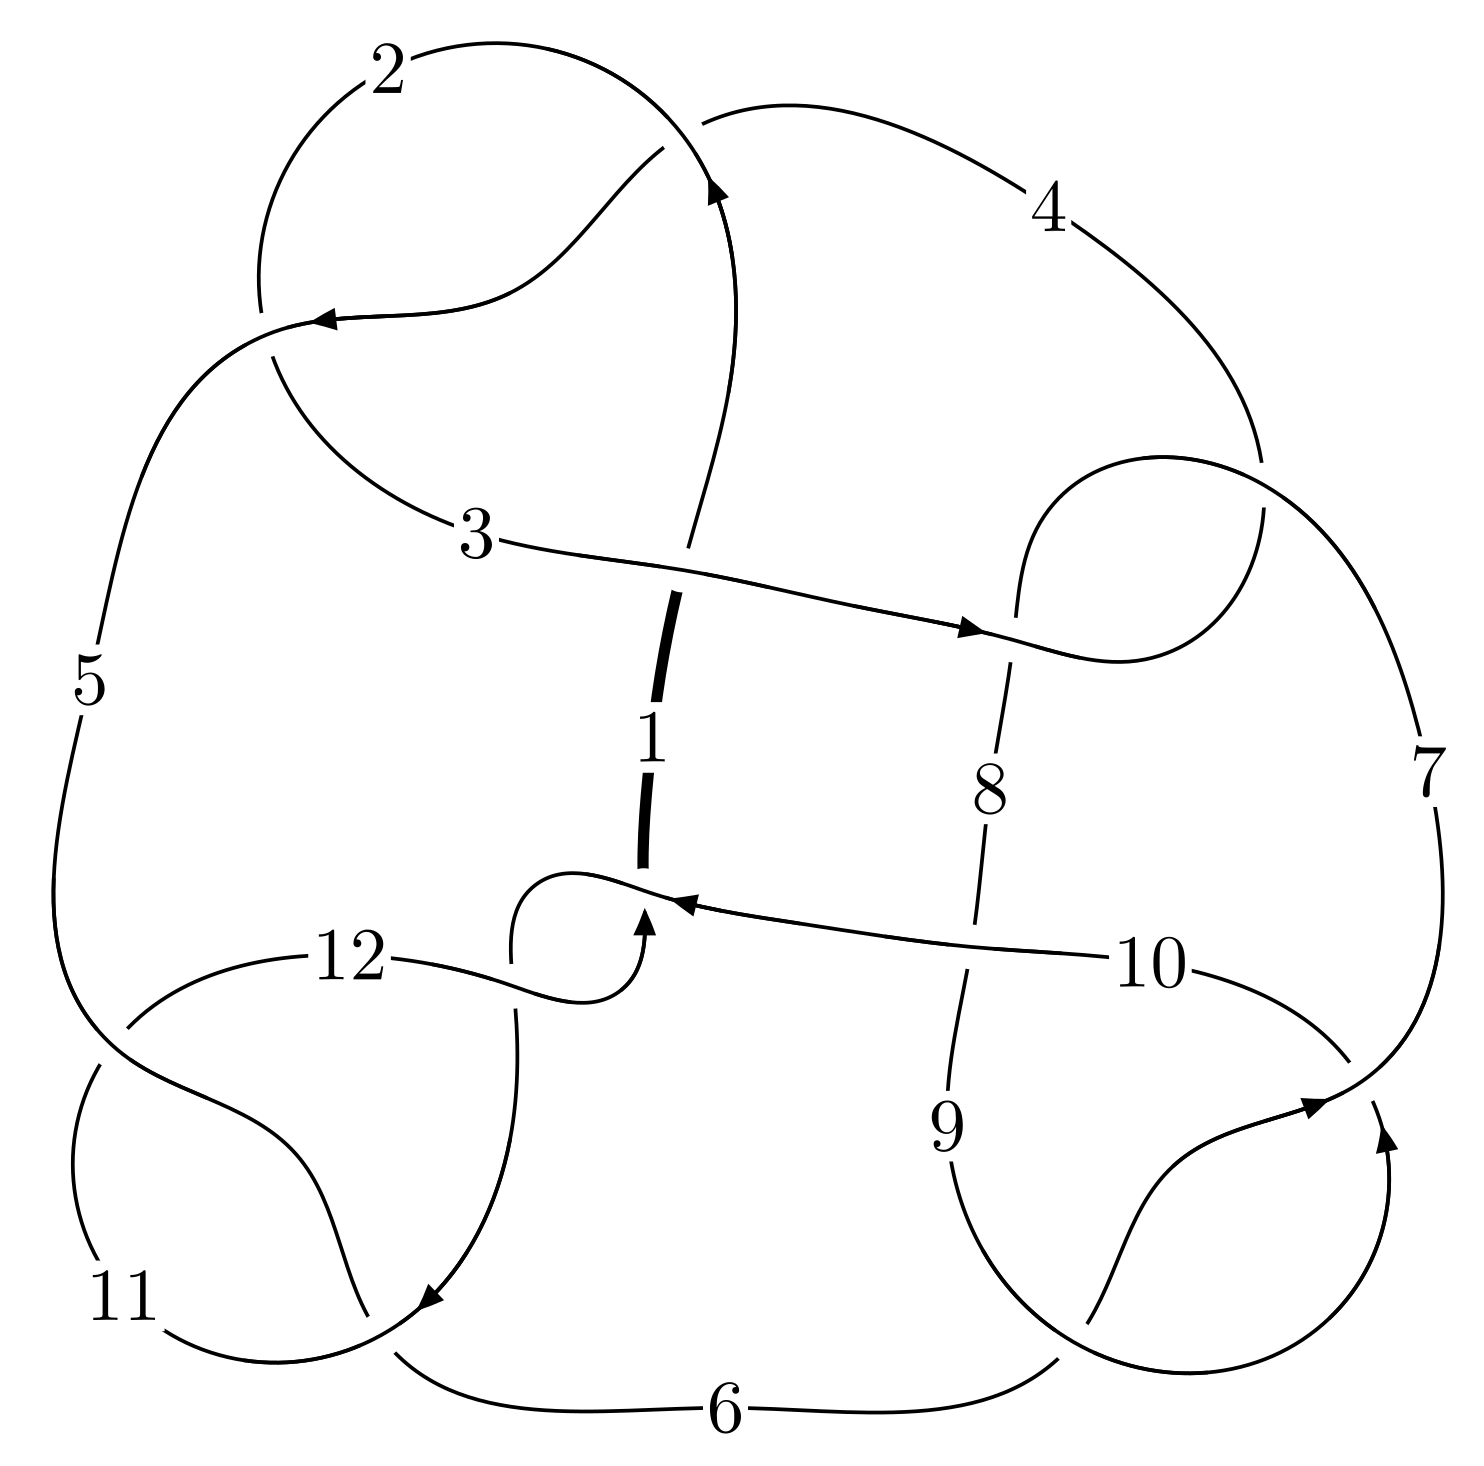
\includegraphics[width=112pt]{../../../GIT/diagram.site/Diagrams/png/2314_12n_0225.png}\\
\ \ \ A knot diagram\footnotemark}&
\allowdisplaybreaks
\textbf{Linearized knot diagam} \\
\cline{2-2}
 &
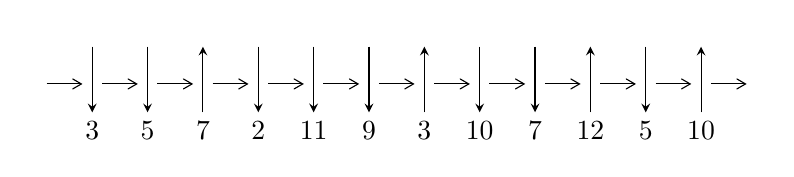
\begin{tikzpicture}[x=20pt, y=17pt]
	% nodes
	\node (C0) at (0, 0) {};
	\node (C1) at (1, 0) {};
	\node (C1U) at (1, +1) {};
	\node (C1D) at (1, -1) {3};

	\node (C2) at (2, 0) {};
	\node (C2U) at (2, +1) {};
	\node (C2D) at (2, -1) {5};

	\node (C3) at (3, 0) {};
	\node (C3U) at (3, +1) {};
	\node (C3D) at (3, -1) {7};

	\node (C4) at (4, 0) {};
	\node (C4U) at (4, +1) {};
	\node (C4D) at (4, -1) {2};

	\node (C5) at (5, 0) {};
	\node (C5U) at (5, +1) {};
	\node (C5D) at (5, -1) {11};

	\node (C6) at (6, 0) {};
	\node (C6U) at (6, +1) {};
	\node (C6D) at (6, -1) {9};

	\node (C7) at (7, 0) {};
	\node (C7U) at (7, +1) {};
	\node (C7D) at (7, -1) {3};

	\node (C8) at (8, 0) {};
	\node (C8U) at (8, +1) {};
	\node (C8D) at (8, -1) {10};

	\node (C9) at (9, 0) {};
	\node (C9U) at (9, +1) {};
	\node (C9D) at (9, -1) {7};

	\node (C10) at (10, 0) {};
	\node (C10U) at (10, +1) {};
	\node (C10D) at (10, -1) {12};

	\node (C11) at (11, 0) {};
	\node (C11U) at (11, +1) {};
	\node (C11D) at (11, -1) {5};

	\node (C12) at (12, 0) {};
	\node (C12U) at (12, +1) {};
	\node (C12D) at (12, -1) {10};
	\node (C13) at (13, 0) {};

	% arrows
	\draw[->,>={angle 60}]
	(C0) edge (C1) (C1) edge (C2) (C2) edge (C3) (C3) edge (C4) (C4) edge (C5) (C5) edge (C6) (C6) edge (C7) (C7) edge (C8) (C8) edge (C9) (C9) edge (C10) (C10) edge (C11) (C11) edge (C12) (C12) edge (C13) ;	\draw[->,>=stealth]
	(C1U) edge (C1D) (C2U) edge (C2D) (C3D) edge (C3U) (C4U) edge (C4D) (C5U) edge (C5D) (C6U) edge (C6D) (C7D) edge (C7U) (C8U) edge (C8D) (C9U) edge (C9D) (C10D) edge (C10U) (C11U) edge (C11D) (C12D) edge (C12U) ;
	\end{tikzpicture} \\
\hhline{~~} \\& 
\textbf{Solving Sequence} \\ \cline{2-2} 
 &
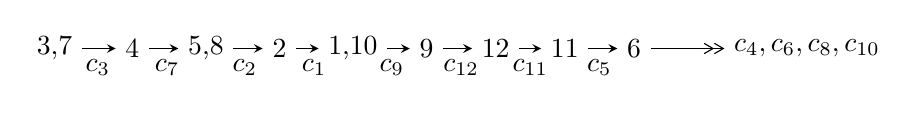
\begin{tikzpicture}[x=25pt, y=7pt]
	% node
	\node (A0) at (-1/8, 0) {3,7};
	\node (A1) at (1, 0) {4};
	\node (A2) at (33/16, 0) {5,8};
	\node (A3) at (25/8, 0) {2};
	\node (A4) at (67/16, 0) {1,10};
	\node (A5) at (21/4, 0) {9};
	\node (A6) at (25/4, 0) {12};
	\node (A7) at (29/4, 0) {11};
	\node (A8) at (33/4, 0) {6};
	\node (C1) at (1/2, -1) {$c_{3}$};
	\node (C2) at (3/2, -1) {$c_{7}$};
	\node (C3) at (21/8, -1) {$c_{2}$};
	\node (C4) at (29/8, -1) {$c_{1}$};
	\node (C5) at (19/4, -1) {$c_{9}$};
	\node (C6) at (23/4, -1) {$c_{12}$};
	\node (C7) at (27/4, -1) {$c_{11}$};
	\node (C8) at (31/4, -1) {$c_{5}$};
	\node (A9) at (43/4, 0) {$c_{4},c_{6},c_{8},c_{10}$};

	% edge
	\draw[->,>=stealth]	
	(A0) edge (A1) (A1) edge (A2) (A2) edge (A3) (A3) edge (A4) (A4) edge (A5) (A5) edge (A6) (A6) edge (A7) (A7) edge (A8) ;
	\draw[->>,>={angle 60}]	
	(A8) edge (A9);
\end{tikzpicture} \\ 

\end{tabular} \\

\footnotetext{
The image of knot diagram is generated by the software ``\textbf{Draw programme}" developed by Andrew Bartholomew(\url{http://www.layer8.co.uk/maths/draw/index.htm\#Running-draw}), where we modified some parts for our purpose(\url{https://github.com/CATsTAILs/LinksPainter}).
}\phantom \\ \newline 
\centering \textbf{Ideals for irreducible components\footnotemark of $X_{\text{par}}$} 
 
\begin{align*}
I^u_{1}&=\langle 
-108733460839492 u^{15}+235633173020139 u^{14}+\cdots+44568754122034192 d-655346094957840,\\
\phantom{I^u_{1}}&\phantom{= \langle  }-5.82443\times10^{14} u^{15}+2.17023\times10^{15} u^{14}+\cdots+8.91375\times10^{16} c+4.50759\times10^{16},\\
\phantom{I^u_{1}}&\phantom{= \langle  }-2.11450\times10^{14} u^{15}+6.65971\times10^{14} u^{14}+\cdots+4.45688\times10^{16} b-9.31909\times10^{15},\\
\phantom{I^u_{1}}&\phantom{= \langle  }40959130934865 u^{15}-340344314483579 u^{14}+\cdots+89137508244068384 a-71636506057825568,\\
\phantom{I^u_{1}}&\phantom{= \langle  }u^{16}-3 u^{15}+\cdots-64 u+32\rangle \\
I^u_{2}&=\langle 
-2059 u^7-2277 u^6+\cdots+6184 d+18886,\;1033 u^7 a-1546 u^7+\cdots-5850 a+12368,\\
\phantom{I^u_{2}}&\phantom{= \langle  }-109 u^7 a+121 u^7+\cdots+2066 a-3882,\;9443 u^7 a-4639 u^7+\cdots-14966 a+1182,\\
\phantom{I^u_{2}}&\phantom{= \langle  }u^8+u^7-7 u^6-4 u^5+16 u^4-3 u^3-9 u^2-8 u-4\rangle \\
\\
I^v_{1}&=\langle 
a,\;d,\;c- v,\;b-1,\;v^2- v+1\rangle \\
I^v_{2}&=\langle 
c,\;d+v-1,\;b,\;a-1,\;v^2- v+1\rangle \\
I^v_{3}&=\langle 
a,\;d+1,\;c+a,\;b-1,\;v+1\rangle \\
I^v_{4}&=\langle 
a,\;a^2 d+c^2 v-2 c a- c v+a+v,\;d v-1,\;c^2 v^2-2 c a v- v^2 c+a^2+a v+v^2,\;b-1\rangle \\
\end{align*}
\raggedright * 5 irreducible components of $\dim_{\mathbb{C}}=0$, with total 37 representations.\\
\raggedright * 1 irreducible components of $\dim_{\mathbb{C}}=1$ \\
\footnotetext{All coefficients of polynomials are rational numbers. But the coefficients are sometimes approximated in decimal forms when there is not enough margin.}
\newpage
\renewcommand{\arraystretch}{1}
\centering \section*{I. $I^u_{1}= \langle -1.09\times10^{14} u^{15}+2.36\times10^{14} u^{14}+\cdots+4.46\times10^{16} d-6.55\times10^{14},\;-5.82\times10^{14} u^{15}+2.17\times10^{15} u^{14}+\cdots+8.91\times10^{16} c+4.51\times10^{16},\;-2.11\times10^{14} u^{15}+6.66\times10^{14} u^{14}+\cdots+4.46\times10^{16} b-9.32\times10^{15},\;4.10\times10^{13} u^{15}-3.40\times10^{14} u^{14}+\cdots+8.91\times10^{16} a-7.16\times10^{16},\;u^{16}-3 u^{15}+\cdots-64 u+32 \rangle$}
\flushleft \textbf{(i) Arc colorings}\\
\begin{tabular}{m{7pt} m{180pt} m{7pt} m{180pt} }
\flushright $a_{3}=$&$\begin{pmatrix}1\\0\end{pmatrix}$ \\
\flushright $a_{7}=$&$\begin{pmatrix}0\\u\end{pmatrix}$ \\
\flushright $a_{4}=$&$\begin{pmatrix}1\\- u^2\end{pmatrix}$ \\
\flushright $a_{5}=$&$\begin{pmatrix}-0.000459505 u^{15}+0.00381819 u^{14}+\cdots+0.107302 u+0.803663\\0.00474436 u^{15}-0.0149425 u^{14}+\cdots+0.0874996 u+0.209095\end{pmatrix}$ \\
\flushright $a_{8}=$&$\begin{pmatrix}u\\u\end{pmatrix}$ \\
\flushright $a_{2}=$&$\begin{pmatrix}-0.000459505 u^{15}+0.00381819 u^{14}+\cdots+0.107302 u+0.803663\\-0.00677644 u^{15}+0.0186134 u^{14}+\cdots-0.258343 u-0.131025\end{pmatrix}$ \\
\flushright $a_{1}=$&$\begin{pmatrix}-0.00723595 u^{15}+0.0224316 u^{14}+\cdots-0.151041 u+0.672638\\-0.00677644 u^{15}+0.0186134 u^{14}+\cdots-0.258343 u-0.131025\end{pmatrix}$ \\
\flushright $a_{10}=$&$\begin{pmatrix}0.00653421 u^{15}-0.0243470 u^{14}+\cdots+2.83891 u-0.505689\\0.00243968 u^{15}-0.00528696 u^{14}+\cdots+0.774255 u+0.0147042\end{pmatrix}$ \\
\flushright $a_{9}=$&$\begin{pmatrix}0.00653421 u^{15}-0.0243470 u^{14}+\cdots+2.83891 u-0.505689\\0.00173022 u^{15}-0.00528404 u^{14}+\cdots+1.28699 u-0.137115\end{pmatrix}$ \\
\flushright $a_{12}=$&$\begin{pmatrix}-0.0137698 u^{15}+0.0405121 u^{14}+\cdots+0.840506 u-0.270168\\-0.00358475 u^{15}+0.0138882 u^{14}+\cdots+0.0905304 u-0.518106\end{pmatrix}$ \\
\flushright $a_{11}=$&$\begin{pmatrix}0.00162230 u^{15}+0.00210951 u^{14}+\cdots+0.961532 u-0.579761\\-0.00282285 u^{15}+0.0157954 u^{14}+\cdots-0.870510 u+0.171332\end{pmatrix}$ \\
\flushright $a_{6}=$&$\begin{pmatrix}0.00409453 u^{15}-0.0190600 u^{14}+\cdots+2.06466 u-0.520393\\-0.000723742 u^{15}-0.00139819 u^{14}+\cdots-0.209537 u-0.231550\end{pmatrix}$\\&\end{tabular}
\flushleft \textbf{(ii) Obstruction class $= -1$}\\~\\
\flushleft \textbf{(iii) Cusp Shapes $= -\frac{3870228309913117}{22284377061017096} u^{15}+\frac{2739800330771103}{5571094265254274} u^{14}+\cdots-\frac{43609984858099500}{2785547132627137} u-\frac{900447030377212}{2785547132627137}$}\\~\\
\newpage\renewcommand{\arraystretch}{1}
\flushleft \textbf{(iv) u-Polynomials at the component}\newline \\
\begin{tabular}{m{50pt}|m{274pt}}
Crossings & \hspace{64pt}u-Polynomials at each crossing \\
\hline $$\begin{aligned}c_{1},c_{8}\end{aligned}$$&$\begin{aligned}
&u^{16}+u^{15}+\cdots-9 u+1
\end{aligned}$\\
\hline $$\begin{aligned}c_{2},c_{4},c_{6}\\c_{9}\end{aligned}$$&$\begin{aligned}
&u^{16}-5 u^{15}+\cdots- u+1
\end{aligned}$\\
\hline $$\begin{aligned}c_{3},c_{7}\end{aligned}$$&$\begin{aligned}
&u^{16}-3 u^{15}+\cdots-64 u+32
\end{aligned}$\\
\hline $$\begin{aligned}c_{5},c_{11}\end{aligned}$$&$\begin{aligned}
&u^{16}- u^{15}+\cdots+8 u+4
\end{aligned}$\\
\hline $$\begin{aligned}c_{10},c_{12}\end{aligned}$$&$\begin{aligned}
&u^{16}-9 u^{15}+\cdots+24 u+16
\end{aligned}$\\
\hline
\end{tabular}\\~\\
\newpage\renewcommand{\arraystretch}{1}
\flushleft \textbf{(v) Riley Polynomials at the component}\newline \\
\begin{tabular}{m{50pt}|m{274pt}}
Crossings & \hspace{64pt}Riley Polynomials at each crossing \\
\hline $$\begin{aligned}c_{1},c_{8}\end{aligned}$$&$\begin{aligned}
&y^{16}+39 y^{15}+\cdots+25 y+1
\end{aligned}$\\
\hline $$\begin{aligned}c_{2},c_{4},c_{6}\\c_{9}\end{aligned}$$&$\begin{aligned}
&y^{16}- y^{15}+\cdots+9 y+1
\end{aligned}$\\
\hline $$\begin{aligned}c_{3},c_{7}\end{aligned}$$&$\begin{aligned}
&y^{16}-15 y^{15}+\cdots+5120 y+1024
\end{aligned}$\\
\hline $$\begin{aligned}c_{5},c_{11}\end{aligned}$$&$\begin{aligned}
&y^{16}+9 y^{15}+\cdots-24 y+16
\end{aligned}$\\
\hline $$\begin{aligned}c_{10},c_{12}\end{aligned}$$&$\begin{aligned}
&y^{16}-3 y^{15}+\cdots+1248 y+256
\end{aligned}$\\
\hline
\end{tabular}\\~\\
\newpage\flushleft \textbf{(vi) Complex Volumes and Cusp Shapes}
$$\begin{array}{c|c|c}  
\text{Solutions to }I^u_{1}& \I (\text{vol} + \sqrt{-1}CS) & \text{Cusp shape}\\
 \hline 
\begin{aligned}
u &= \phantom{-}0.289911 + 0.801405 I \\
a &= \phantom{-}0.654021 + 0.248004 I \\
b &= \phantom{-}0.336785 - 0.506907 I \\
c &= \phantom{-}0.424894 + 0.573951 I \\
d &= -0.009143 + 0.596034 I\end{aligned}
 & -0.321814 + 1.225450 I & -4.70206 - 4.90073 I \\ \hline\begin{aligned}
u &= \phantom{-}0.289911 - 0.801405 I \\
a &= \phantom{-}0.654021 - 0.248004 I \\
b &= \phantom{-}0.336785 + 0.506907 I \\
c &= \phantom{-}0.424894 - 0.573951 I \\
d &= -0.009143 - 0.596034 I\end{aligned}
 & -0.321814 - 1.225450 I & -4.70206 + 4.90073 I \\ \hline\begin{aligned}
u &= -1.139570 + 0.424244 I \\
a &= \phantom{-}0.589120 - 0.792720 I \\
b &= -0.396064 + 0.812657 I \\
c &= -0.538420 + 0.512682 I \\
d &= -0.335035 + 1.153290 I\end{aligned}
 & \phantom{-}0.71555 + 3.67228 I & -1.72542 - 4.33532 I \\ \hline\begin{aligned}
u &= -1.139570 - 0.424244 I \\
a &= \phantom{-}0.589120 + 0.792720 I \\
b &= -0.396064 - 0.812657 I \\
c &= -0.538420 - 0.512682 I \\
d &= -0.335035 - 1.153290 I\end{aligned}
 & \phantom{-}0.71555 - 3.67228 I & -1.72542 + 4.33532 I \\ \hline\begin{aligned}
u &= \phantom{-}0.575594 + 0.321074 I \\
a &= \phantom{-}1.017480 + 0.434986 I \\
b &= -0.169050 - 0.355242 I \\
c &= \phantom{-}0.486567 + 0.345761 I \\
d &= \phantom{-}0.445993 + 0.577062 I\end{aligned}
 & -0.11872 + 1.44911 I & \phantom{-}0.36516 - 2.80335 I \\ \hline\begin{aligned}
u &= \phantom{-}0.575594 - 0.321074 I \\
a &= \phantom{-}1.017480 - 0.434986 I \\
b &= -0.169050 + 0.355242 I \\
c &= \phantom{-}0.486567 - 0.345761 I \\
d &= \phantom{-}0.445993 - 0.577062 I\end{aligned}
 & -0.11872 - 1.44911 I & \phantom{-}0.36516 + 2.80335 I\\
 \hline 
 \end{array}$$\newpage$$\begin{array}{c|c|c}  
\text{Solutions to }I^u_{1}& \I (\text{vol} + \sqrt{-1}CS) & \text{Cusp shape}\\
 \hline 
\begin{aligned}
u &= -0.067191 + 0.531573 I \\
a &= \phantom{-}0.547892 + 0.020957 I \\
b &= \phantom{-}0.822510 - 0.069711 I \\
c &= \phantom{-}0.32158 + 1.50666 I \\
d &= -0.047954 + 0.289837 I\end{aligned}
 & -2.85279 + 2.27613 I & -11.67196 - 3.94896 I \\ \hline\begin{aligned}
u &= -0.067191 - 0.531573 I \\
a &= \phantom{-}0.547892 - 0.020957 I \\
b &= \phantom{-}0.822510 + 0.069711 I \\
c &= \phantom{-}0.32158 - 1.50666 I \\
d &= -0.047954 - 0.289837 I\end{aligned}
 & -2.85279 - 2.27613 I & -11.67196 + 3.94896 I \\ \hline\begin{aligned}
u &= -0.33229 + 1.72297 I \\
a &= \phantom{-}0.412801 - 0.282825 I \\
b &= \phantom{-}0.648602 + 1.129520 I \\
c &= -0.562057 + 0.484841 I \\
d &= \phantom{-}0.350130 + 0.805225 I\end{aligned}
 & \phantom{-}4.26031 - 4.58330 I & -1.71878 + 4.05752 I \\ \hline\begin{aligned}
u &= -0.33229 - 1.72297 I \\
a &= \phantom{-}0.412801 + 0.282825 I \\
b &= \phantom{-}0.648602 - 1.129520 I \\
c &= -0.562057 - 0.484841 I \\
d &= \phantom{-}0.350130 - 0.805225 I\end{aligned}
 & \phantom{-}4.26031 + 4.58330 I & -1.71878 - 4.05752 I \\ \hline\begin{aligned}
u &= -1.81588 + 0.68377 I \\
a &= -0.227904 + 0.980118 I \\
b &= -1.22507 - 0.96795 I \\
c &= -0.415075 - 0.689342 I \\
d &= -0.25632 - 1.93561 I\end{aligned}
 & \phantom{-}6.64229 - 8.00732 I & -6.00576 + 3.88395 I \\ \hline\begin{aligned}
u &= -1.81588 - 0.68377 I \\
a &= -0.227904 - 0.980118 I \\
b &= -1.22507 + 0.96795 I \\
c &= -0.415075 + 0.689342 I \\
d &= -0.25632 + 1.93561 I\end{aligned}
 & \phantom{-}6.64229 + 8.00732 I & -6.00576 - 3.88395 I\\
 \hline 
 \end{array}$$\newpage$$\begin{array}{c|c|c}  
\text{Solutions to }I^u_{1}& \I (\text{vol} + \sqrt{-1}CS) & \text{Cusp shape}\\
 \hline 
\begin{aligned}
u &= \phantom{-}1.72439 + 0.95526 I \\
a &= -0.389017 - 0.972862 I \\
b &= -1.35436 + 0.88620 I \\
c &= \phantom{-}0.383140 - 0.726169 I \\
d &= \phantom{-}0.25852 - 2.04920 I\end{aligned}
 & \phantom{-}9.8252 + 14.1242 I & -4.39428 - 6.97100 I \\ \hline\begin{aligned}
u &= \phantom{-}1.72439 - 0.95526 I \\
a &= -0.389017 + 0.972862 I \\
b &= -1.35436 - 0.88620 I \\
c &= \phantom{-}0.383140 + 0.726169 I \\
d &= \phantom{-}0.25852 + 2.04920 I\end{aligned}
 & \phantom{-}9.8252 - 14.1242 I & -4.39428 + 6.97100 I \\ \hline\begin{aligned}
u &= \phantom{-}2.26504 + 0.41669 I \\
a &= -0.104392 - 0.792584 I \\
b &= -1.16335 + 1.24018 I \\
c &= \phantom{-}0.399366 - 0.621003 I \\
d &= \phantom{-}0.09381 - 1.83873 I\end{aligned}
 & \phantom{-}12.28130 + 3.00558 I & -2.14690 - 1.40998 I \\ \hline\begin{aligned}
u &= \phantom{-}2.26504 - 0.41669 I \\
a &= -0.104392 + 0.792584 I \\
b &= -1.16335 - 1.24018 I \\
c &= \phantom{-}0.399366 + 0.621003 I \\
d &= \phantom{-}0.09381 + 1.83873 I\end{aligned}
 & \phantom{-}12.28130 - 3.00558 I & -2.14690 + 1.40998 I\\
 \hline 
 \end{array}$$\newpage\newpage\renewcommand{\arraystretch}{1}
\centering \section*{II. $I^u_{2}= \langle -2059 u^{7}-2277 u^{6}+\cdots+6184 d+1.89\times10^{4},\;1033 a u^{7}-1546 u^{7}+\cdots-5850 a+1.24\times10^{4},\;-109 a u^{7}+121 u^{7}+\cdots+2066 a-3882,\;9443 a u^{7}-4639 u^{7}+\cdots-1.50\times10^{4} a+1182,\;u^8+u^7+\cdots-8 u-4 \rangle$}
\flushleft \textbf{(i) Arc colorings}\\
\begin{tabular}{m{7pt} m{180pt} m{7pt} m{180pt} }
\flushright $a_{3}=$&$\begin{pmatrix}1\\0\end{pmatrix}$ \\
\flushright $a_{7}=$&$\begin{pmatrix}0\\u\end{pmatrix}$ \\
\flushright $a_{4}=$&$\begin{pmatrix}1\\- u^2\end{pmatrix}$ \\
\flushright $a_{5}=$&$\begin{pmatrix}a\\0.0352523 a u^{7}-0.0391332 u^{7}+\cdots-0.668176 a+1.25550\end{pmatrix}$ \\
\flushright $a_{8}=$&$\begin{pmatrix}u\\u\end{pmatrix}$ \\
\flushright $a_{2}=$&$\begin{pmatrix}a\\-0.0352523 a u^{7}+0.0391332 u^{7}+\cdots+0.668176 a-1.25550\end{pmatrix}$ \\
\flushright $a_{1}=$&$\begin{pmatrix}-0.0352523 a u^{7}+0.0391332 u^{7}+\cdots+1.66818 a-1.25550\\-0.0352523 a u^{7}+0.0391332 u^{7}+\cdots+0.668176 a-1.25550\end{pmatrix}$ \\
\flushright $a_{10}=$&$\begin{pmatrix}-\frac{1033}{6184} u^7 a+\frac{1}{4} u^7+\cdots+\frac{2925}{3092} a-2\\0.332956 u^{7}+0.368208 u^{6}+\cdots-4.89796 u-3.05401\end{pmatrix}$ \\
\flushright $a_{9}=$&$\begin{pmatrix}-\frac{1033}{6184} u^7 a+\frac{1}{4} u^7+\cdots+\frac{2925}{3092} a-2\\0.150712 a u^{7}+0.332956 u^{7}+\cdots-0.141009 a-3.05401\end{pmatrix}$ \\
\flushright $a_{12}=$&$\begin{pmatrix}-0.0391332 a u^{7}+0.0133409 u^{7}+\cdots+1.25550 a-2.01892\\-0.0187581 a u^{7}-0.0163325 u^{7}+\cdots+0.172057 a-3.19502\end{pmatrix}$ \\
\flushright $a_{11}=$&$\begin{pmatrix}-0.0163325 a u^{7}+0.0133409 u^{7}+\cdots+0.804981 a-2.01892\\-0.00226391 a u^{7}-0.0593467 u^{7}+\cdots-0.324062 a-3.35220\end{pmatrix}$ \\
\flushright $a_{6}=$&$\begin{pmatrix}-0.167044 a u^{7}-0.0829560 u^{7}+\cdots+0.945990 a+1.05401\\0.150712 a u^{7}-0.483668 u^{7}+\cdots-0.141009 a+3.19502\end{pmatrix}$\\&\end{tabular}
\flushleft \textbf{(ii) Obstruction class $= -1$}\\~\\
\flushleft \textbf{(iii) Cusp Shapes $= -\frac{933}{1546} u^7-\frac{561}{1546} u^6+\frac{7043}{1546} u^5+\frac{278}{773} u^4-\frac{8922}{773} u^3+\frac{11743}{1546} u^2+\frac{10913}{1546} u-\frac{2838}{773}$}\\~\\
\newpage\renewcommand{\arraystretch}{1}
\flushleft \textbf{(iv) u-Polynomials at the component}\newline \\
\begin{tabular}{m{50pt}|m{274pt}}
Crossings & \hspace{64pt}u-Polynomials at each crossing \\
\hline $$\begin{aligned}c_{1},c_{8}\end{aligned}$$&$\begin{aligned}
&u^{16}+3 u^{15}+\cdots+2336 u+256
\end{aligned}$\\
\hline $$\begin{aligned}c_{2},c_{4},c_{6}\\c_{9}\end{aligned}$$&$\begin{aligned}
&u^{16}-3 u^{15}+\cdots+40 u-16
\end{aligned}$\\
\hline $$\begin{aligned}c_{3},c_{7}\end{aligned}$$&$\begin{aligned}
&(u^8+u^7-7 u^6-4 u^5+16 u^4-3 u^3-9 u^2-8 u-4)^2
\end{aligned}$\\
\hline $$\begin{aligned}c_{5},c_{11}\end{aligned}$$&$\begin{aligned}
&(u^8-2 u^7+5 u^6-6 u^5+7 u^4-7 u^3+4 u^2-4 u+1)^2
\end{aligned}$\\
\hline $$\begin{aligned}c_{10},c_{12}\end{aligned}$$&$\begin{aligned}
&(u^8-6 u^7+15 u^6-14 u^5-9 u^4+31 u^3-26 u^2+8 u+1)^2
\end{aligned}$\\
\hline
\end{tabular}\\~\\
\newpage\renewcommand{\arraystretch}{1}
\flushleft \textbf{(v) Riley Polynomials at the component}\newline \\
\begin{tabular}{m{50pt}|m{274pt}}
Crossings & \hspace{64pt}Riley Polynomials at each crossing \\
\hline $$\begin{aligned}c_{1},c_{8}\end{aligned}$$&$\begin{aligned}
&y^{16}+17 y^{15}+\cdots-2843136 y+65536
\end{aligned}$\\
\hline $$\begin{aligned}c_{2},c_{4},c_{6}\\c_{9}\end{aligned}$$&$\begin{aligned}
&y^{16}-3 y^{15}+\cdots-2336 y+256
\end{aligned}$\\
\hline $$\begin{aligned}c_{3},c_{7}\end{aligned}$$&$\begin{aligned}
&(y^8-15 y^7+89 y^6-252 y^5+366 y^4-305 y^3-95 y^2+8 y+16)^2
\end{aligned}$\\
\hline $$\begin{aligned}c_{5},c_{11}\end{aligned}$$&$\begin{aligned}
&(y^8+6 y^7+15 y^6+14 y^5-9 y^4-31 y^3-26 y^2-8 y+1)^2
\end{aligned}$\\
\hline $$\begin{aligned}c_{10},c_{12}\end{aligned}$$&$\begin{aligned}
&(y^8-6 y^7+39 y^6-146 y^5+267 y^4-239 y^3+162 y^2-116 y+1)^2
\end{aligned}$\\
\hline
\end{tabular}\\~\\
\newpage\flushleft \textbf{(vi) Complex Volumes and Cusp Shapes}
$$\begin{array}{c|c|c}  
\text{Solutions to }I^u_{2}& \I (\text{vol} + \sqrt{-1}CS) & \text{Cusp shape}\\
 \hline 
\begin{aligned}
u &= \phantom{-}1.170290 + 0.725937 I \\
a &= \phantom{-}0.508470 + 0.631641 I \\
b &= -0.226676 - 0.960653 I \\
c &= -1.002720 + 0.319564 I \\
d &= \phantom{-}0.519668 + 0.225325 I\end{aligned}
 & \phantom{-}1.14222 - 1.62541 I & -1.41499 + 1.42555 I \\ \hline\begin{aligned}
u &= \phantom{-}1.170290 + 0.725937 I \\
a &= \phantom{-}0.406912 - 0.059872 I \\
b &= \phantom{-}1.40546 + 0.35393 I \\
c &= \phantom{-}0.507576 + 0.506015 I \\
d &= \phantom{-}0.136526 + 1.108320 I\end{aligned}
 & \phantom{-}1.14222 - 1.62541 I & -1.41499 + 1.42555 I \\ \hline\begin{aligned}
u &= \phantom{-}1.170290 - 0.725937 I \\
a &= \phantom{-}0.508470 - 0.631641 I \\
b &= -0.226676 + 0.960653 I \\
c &= -1.002720 - 0.319564 I \\
d &= \phantom{-}0.519668 - 0.225325 I\end{aligned}
 & \phantom{-}1.14222 + 1.62541 I & -1.41499 - 1.42555 I \\ \hline\begin{aligned}
u &= \phantom{-}1.170290 - 0.725937 I \\
a &= \phantom{-}0.406912 + 0.059872 I \\
b &= \phantom{-}1.40546 - 0.35393 I \\
c &= \phantom{-}0.507576 - 0.506015 I \\
d &= \phantom{-}0.136526 - 1.108320 I\end{aligned}
 & \phantom{-}1.14222 + 1.62541 I & -1.41499 - 1.42555 I \\ \hline\begin{aligned}
u &= -0.195492 + 0.552709 I \\
a &= \phantom{-}0.527146 + 0.046214 I \\
b &= \phantom{-}0.882537 - 0.165040 I \\
c &= -0.51191 - 1.84722 I \\
d &= -0.94136 - 3.95806 I\end{aligned}
 & -2.92647 - 1.66195 I & -9.38368 + 3.48117 I \\ \hline\begin{aligned}
u &= -0.195492 + 0.552709 I \\
a &= -5.82950 + 3.76506 I \\
b &= -1.121050 - 0.078180 I \\
c &= \phantom{-}0.76737 + 1.32533 I \\
d &= -0.128596 + 0.282324 I\end{aligned}
 & -2.92647 - 1.66195 I & -9.38368 + 3.48117 I\\
 \hline 
 \end{array}$$\newpage$$\begin{array}{c|c|c}  
\text{Solutions to }I^u_{2}& \I (\text{vol} + \sqrt{-1}CS) & \text{Cusp shape}\\
 \hline 
\begin{aligned}
u &= -0.195492 - 0.552709 I \\
a &= \phantom{-}0.527146 - 0.046214 I \\
b &= \phantom{-}0.882537 + 0.165040 I \\
c &= -0.51191 + 1.84722 I \\
d &= -0.94136 + 3.95806 I\end{aligned}
 & -2.92647 + 1.66195 I & -9.38368 - 3.48117 I \\ \hline\begin{aligned}
u &= -0.195492 - 0.552709 I \\
a &= -5.82950 - 3.76506 I \\
b &= -1.121050 + 0.078180 I \\
c &= \phantom{-}0.76737 - 1.32533 I \\
d &= -0.128596 - 0.282324 I\end{aligned}
 & -2.92647 + 1.66195 I & -9.38368 - 3.48117 I \\ \hline\begin{aligned}
u &= -0.580387\phantom{ +0.000000I} \\
a &= \phantom{-}0.467644\phantom{ +0.000000I} \\
b &= \phantom{-}1.13838\phantom{ +0.000000I} \\
c &= -0.692019\phantom{ +0.000000I} \\
d &= -0.969961\phantom{ +0.000000I}\end{aligned}
 & -2.18625\phantom{ +0.000000I} & -3.21290\phantom{ +0.000000I} \\ \hline\begin{aligned}
u &= -0.580387\phantom{ +0.000000I} \\
a &= \phantom{-}1.67123\phantom{ +0.000000I} \\
b &= -0.401639\phantom{ +0.000000I} \\
c &= \phantom{-}1.96141\phantom{ +0.000000I} \\
d &= -0.271415\phantom{ +0.000000I}\end{aligned}
 & -2.18625\phantom{ +0.000000I} & -3.21290\phantom{ +0.000000I} \\ \hline\begin{aligned}
u &= \phantom{-}2.05532\phantom{ +0.000000I} \\
a &= \phantom{-}0.059530 + 0.815129 I \\
b &= -0.91088 - 1.22029 I \\
c &= \phantom{-}0.443183 - 0.593724 I \\
d &= \phantom{-}0.12235 - 1.67535 I\end{aligned}
 & \phantom{-}7.78143\phantom{ +0.000000I} & -4.64060\phantom{ +0.000000I} \\ \hline\begin{aligned}
u &= \phantom{-}2.05532\phantom{ +0.000000I} \\
a &= \phantom{-}0.059530 - 0.815129 I \\
b &= -0.91088 + 1.22029 I \\
c &= \phantom{-}0.443183 + 0.593724 I \\
d &= \phantom{-}0.12235 + 1.67535 I\end{aligned}
 & \phantom{-}7.78143\phantom{ +0.000000I} & -4.64060\phantom{ +0.000000I}\\
 \hline 
 \end{array}$$\newpage$$\begin{array}{c|c|c}  
\text{Solutions to }I^u_{2}& \I (\text{vol} + \sqrt{-1}CS) & \text{Cusp shape}\\
 \hline 
\begin{aligned}
u &= -2.21226 + 0.50002 I \\
a &= -0.131998 + 0.812425 I \\
b &= -1.19484 - 1.19923 I \\
c &= -0.440910 + 0.544962 I \\
d &= \phantom{-}0.02631 + 1.55679 I\end{aligned}
 & \phantom{-}12.14610 - 5.90409 I & -2.27459 + 2.82977 I \\ \hline\begin{aligned}
u &= -2.21226 + 0.50002 I \\
a &= \phantom{-}0.140006 - 0.672065 I \\
b &= -0.70292 + 1.42606 I \\
c &= -0.397283 - 0.631875 I \\
d &= -0.11421 - 1.86330 I\end{aligned}
 & \phantom{-}12.14610 - 5.90409 I & -2.27459 + 2.82977 I \\ \hline\begin{aligned}
u &= -2.21226 - 0.50002 I \\
a &= -0.131998 - 0.812425 I \\
b &= -1.19484 + 1.19923 I \\
c &= -0.440910 - 0.544962 I \\
d &= \phantom{-}0.02631 - 1.55679 I\end{aligned}
 & \phantom{-}12.14610 + 5.90409 I & -2.27459 - 2.82977 I \\ \hline\begin{aligned}
u &= -2.21226 - 0.50002 I \\
a &= \phantom{-}0.140006 + 0.672065 I \\
b &= -0.70292 - 1.42606 I \\
c &= -0.397283 + 0.631875 I \\
d &= -0.11421 + 1.86330 I\end{aligned}
 & \phantom{-}12.14610 + 5.90409 I & -2.27459 - 2.82977 I\\
 \hline 
 \end{array}$$\newpage\newpage\renewcommand{\arraystretch}{1}
\centering \section*{III. $I^v_{1}= \langle a,\;d,\;c- v,\;b-1,\;v^2- v+1 \rangle$}
\flushleft \textbf{(i) Arc colorings}\\
\begin{tabular}{m{7pt} m{180pt} m{7pt} m{180pt} }
\flushright $a_{3}=$&$\begin{pmatrix}1\\0\end{pmatrix}$ \\
\flushright $a_{7}=$&$\begin{pmatrix}v\\0\end{pmatrix}$ \\
\flushright $a_{4}=$&$\begin{pmatrix}1\\0\end{pmatrix}$ \\
\flushright $a_{5}=$&$\begin{pmatrix}0\\1\end{pmatrix}$ \\
\flushright $a_{8}=$&$\begin{pmatrix}v\\0\end{pmatrix}$ \\
\flushright $a_{2}=$&$\begin{pmatrix}1\\-1\end{pmatrix}$ \\
\flushright $a_{1}=$&$\begin{pmatrix}0\\-1\end{pmatrix}$ \\
\flushright $a_{10}=$&$\begin{pmatrix}v\\0\end{pmatrix}$ \\
\flushright $a_{9}=$&$\begin{pmatrix}v\\0\end{pmatrix}$ \\
\flushright $a_{12}=$&$\begin{pmatrix}v-1\\-1\end{pmatrix}$ \\
\flushright $a_{11}=$&$\begin{pmatrix}v-1\\- v\end{pmatrix}$ \\
\flushright $a_{6}=$&$\begin{pmatrix}v\\0\end{pmatrix}$\\&\end{tabular}
\flushleft \textbf{(ii) Obstruction class $= 1$}\\~\\
\flushleft \textbf{(iii) Cusp Shapes $= -4 v-1$}\\~\\
\newpage\renewcommand{\arraystretch}{1}
\flushleft \textbf{(iv) u-Polynomials at the component}\newline \\
\begin{tabular}{m{50pt}|m{274pt}}
Crossings & \hspace{64pt}u-Polynomials at each crossing \\
\hline $$\begin{aligned}c_{1},c_{2}\end{aligned}$$&$\begin{aligned}
&(u-1)^2
\end{aligned}$\\
\hline $$\begin{aligned}c_{3},c_{6},c_{7}\\c_{8},c_{9}\end{aligned}$$&$\begin{aligned}
&u^2
\end{aligned}$\\
\hline $$\begin{aligned}c_{4}\end{aligned}$$&$\begin{aligned}
&(u+1)^2
\end{aligned}$\\
\hline $$\begin{aligned}c_{5},c_{12}\end{aligned}$$&$\begin{aligned}
&u^2- u+1
\end{aligned}$\\
\hline $$\begin{aligned}c_{10},c_{11}\end{aligned}$$&$\begin{aligned}
&u^2+u+1
\end{aligned}$\\
\hline
\end{tabular}\\~\\
\newpage\renewcommand{\arraystretch}{1}
\flushleft \textbf{(v) Riley Polynomials at the component}\newline \\
\begin{tabular}{m{50pt}|m{274pt}}
Crossings & \hspace{64pt}Riley Polynomials at each crossing \\
\hline $$\begin{aligned}c_{1},c_{2},c_{4}\end{aligned}$$&$\begin{aligned}
&(y-1)^2
\end{aligned}$\\
\hline $$\begin{aligned}c_{3},c_{6},c_{7}\\c_{8},c_{9}\end{aligned}$$&$\begin{aligned}
&y^2
\end{aligned}$\\
\hline $$\begin{aligned}c_{5},c_{10},c_{11}\\c_{12}\end{aligned}$$&$\begin{aligned}
&y^2+y+1
\end{aligned}$\\
\hline
\end{tabular}\\~\\
\newpage\flushleft \textbf{(vi) Complex Volumes and Cusp Shapes}
$$\begin{array}{c|c|c}  
\text{Solutions to }I^v_{1}& \I (\text{vol} + \sqrt{-1}CS) & \text{Cusp shape}\\
 \hline 
\begin{aligned}
v &= \phantom{-}0.500000 + 0.866025 I \\
a &= \phantom{-0.000000 } 0 \\
b &= \phantom{-}1.00000\phantom{ +0.000000I} \\
c &= \phantom{-}0.500000 + 0.866025 I \\
d &= \phantom{-0.000000 } 0\end{aligned}
 & -1.64493 + 2.02988 I & -3.00000 - 3.46410 I \\ \hline\begin{aligned}
v &= \phantom{-}0.500000 - 0.866025 I \\
a &= \phantom{-0.000000 } 0 \\
b &= \phantom{-}1.00000\phantom{ +0.000000I} \\
c &= \phantom{-}0.500000 - 0.866025 I \\
d &= \phantom{-0.000000 } 0\end{aligned}
 & -1.64493 - 2.02988 I & -3.00000 + 3.46410 I\\
 \hline 
 \end{array}$$\newpage\newpage\renewcommand{\arraystretch}{1}
\centering \section*{IV. $I^v_{2}= \langle c,\;d+v-1,\;b,\;a-1,\;v^2- v+1 \rangle$}
\flushleft \textbf{(i) Arc colorings}\\
\begin{tabular}{m{7pt} m{180pt} m{7pt} m{180pt} }
\flushright $a_{3}=$&$\begin{pmatrix}1\\0\end{pmatrix}$ \\
\flushright $a_{7}=$&$\begin{pmatrix}v\\0\end{pmatrix}$ \\
\flushright $a_{4}=$&$\begin{pmatrix}1\\0\end{pmatrix}$ \\
\flushright $a_{5}=$&$\begin{pmatrix}1\\0\end{pmatrix}$ \\
\flushright $a_{8}=$&$\begin{pmatrix}v\\0\end{pmatrix}$ \\
\flushright $a_{2}=$&$\begin{pmatrix}1\\0\end{pmatrix}$ \\
\flushright $a_{1}=$&$\begin{pmatrix}1\\0\end{pmatrix}$ \\
\flushright $a_{10}=$&$\begin{pmatrix}0\\- v+1\end{pmatrix}$ \\
\flushright $a_{9}=$&$\begin{pmatrix}v\\- v+1\end{pmatrix}$ \\
\flushright $a_{12}=$&$\begin{pmatrix}1\\- v\end{pmatrix}$ \\
\flushright $a_{11}=$&$\begin{pmatrix}- v+1\\- v\end{pmatrix}$ \\
\flushright $a_{6}=$&$\begin{pmatrix}0\\v-1\end{pmatrix}$\\&\end{tabular}
\flushleft \textbf{(ii) Obstruction class $= 1$}\\~\\
\flushleft \textbf{(iii) Cusp Shapes $= 4 v-5$}\\~\\
\newpage\renewcommand{\arraystretch}{1}
\flushleft \textbf{(iv) u-Polynomials at the component}\newline \\
\begin{tabular}{m{50pt}|m{274pt}}
Crossings & \hspace{64pt}u-Polynomials at each crossing \\
\hline $$\begin{aligned}c_{1},c_{2},c_{3}\\c_{4},c_{7}\end{aligned}$$&$\begin{aligned}
&u^2
\end{aligned}$\\
\hline $$\begin{aligned}c_{5},c_{10}\end{aligned}$$&$\begin{aligned}
&u^2+u+1
\end{aligned}$\\
\hline $$\begin{aligned}c_{6},c_{8}\end{aligned}$$&$\begin{aligned}
&(u-1)^2
\end{aligned}$\\
\hline $$\begin{aligned}c_{9}\end{aligned}$$&$\begin{aligned}
&(u+1)^2
\end{aligned}$\\
\hline $$\begin{aligned}c_{11},c_{12}\end{aligned}$$&$\begin{aligned}
&u^2- u+1
\end{aligned}$\\
\hline
\end{tabular}\\~\\
\newpage\renewcommand{\arraystretch}{1}
\flushleft \textbf{(v) Riley Polynomials at the component}\newline \\
\begin{tabular}{m{50pt}|m{274pt}}
Crossings & \hspace{64pt}Riley Polynomials at each crossing \\
\hline $$\begin{aligned}c_{1},c_{2},c_{3}\\c_{4},c_{7}\end{aligned}$$&$\begin{aligned}
&y^2
\end{aligned}$\\
\hline $$\begin{aligned}c_{5},c_{10},c_{11}\\c_{12}\end{aligned}$$&$\begin{aligned}
&y^2+y+1
\end{aligned}$\\
\hline $$\begin{aligned}c_{6},c_{8},c_{9}\end{aligned}$$&$\begin{aligned}
&(y-1)^2
\end{aligned}$\\
\hline
\end{tabular}\\~\\
\newpage\flushleft \textbf{(vi) Complex Volumes and Cusp Shapes}
$$\begin{array}{c|c|c}  
\text{Solutions to }I^v_{2}& \I (\text{vol} + \sqrt{-1}CS) & \text{Cusp shape}\\
 \hline 
\begin{aligned}
v &= \phantom{-}0.500000 + 0.866025 I \\
a &= \phantom{-}1.00000\phantom{ +0.000000I} \\
b &= \phantom{-0.000000 } 0 \\
c &= \phantom{-0.000000 } 0 \\
d &= \phantom{-}0.500000 - 0.866025 I\end{aligned}
 & -1.64493 - 2.02988 I & -3.00000 + 3.46410 I \\ \hline\begin{aligned}
v &= \phantom{-}0.500000 - 0.866025 I \\
a &= \phantom{-}1.00000\phantom{ +0.000000I} \\
b &= \phantom{-0.000000 } 0 \\
c &= \phantom{-0.000000 } 0 \\
d &= \phantom{-}0.500000 + 0.866025 I\end{aligned}
 & -1.64493 + 2.02988 I & -3.00000 - 3.46410 I\\
 \hline 
 \end{array}$$\newpage\newpage\renewcommand{\arraystretch}{1}
\centering \section*{V. $I^v_{3}= \langle a,\;d+1,\;c+a,\;b-1,\;v+1 \rangle$}
\flushleft \textbf{(i) Arc colorings}\\
\begin{tabular}{m{7pt} m{180pt} m{7pt} m{180pt} }
\flushright $a_{3}=$&$\begin{pmatrix}1\\0\end{pmatrix}$ \\
\flushright $a_{7}=$&$\begin{pmatrix}-1\\0\end{pmatrix}$ \\
\flushright $a_{4}=$&$\begin{pmatrix}1\\0\end{pmatrix}$ \\
\flushright $a_{5}=$&$\begin{pmatrix}0\\1\end{pmatrix}$ \\
\flushright $a_{8}=$&$\begin{pmatrix}-1\\0\end{pmatrix}$ \\
\flushright $a_{2}=$&$\begin{pmatrix}1\\-1\end{pmatrix}$ \\
\flushright $a_{1}=$&$\begin{pmatrix}0\\-1\end{pmatrix}$ \\
\flushright $a_{10}=$&$\begin{pmatrix}0\\-1\end{pmatrix}$ \\
\flushright $a_{9}=$&$\begin{pmatrix}-1\\-1\end{pmatrix}$ \\
\flushright $a_{12}=$&$\begin{pmatrix}0\\-1\end{pmatrix}$ \\
\flushright $a_{11}=$&$\begin{pmatrix}0\\-1\end{pmatrix}$ \\
\flushright $a_{6}=$&$\begin{pmatrix}0\\1\end{pmatrix}$\\&\end{tabular}
\flushleft \textbf{(ii) Obstruction class $= 1$}\\~\\
\flushleft \textbf{(iii) Cusp Shapes $= -12$}\\~\\
\newpage\renewcommand{\arraystretch}{1}
\flushleft \textbf{(iv) u-Polynomials at the component}\newline \\
\begin{tabular}{m{50pt}|m{274pt}}
Crossings & \hspace{64pt}u-Polynomials at each crossing \\
\hline $$\begin{aligned}c_{1},c_{2},c_{6}\\c_{8}\end{aligned}$$&$\begin{aligned}
&u-1
\end{aligned}$\\
\hline $$\begin{aligned}c_{3},c_{5},c_{7}\\c_{10},c_{11},c_{12}\end{aligned}$$&$\begin{aligned}
&u
\end{aligned}$\\
\hline $$\begin{aligned}c_{4},c_{9}\end{aligned}$$&$\begin{aligned}
&u+1
\end{aligned}$\\
\hline
\end{tabular}\\~\\
\newpage\renewcommand{\arraystretch}{1}
\flushleft \textbf{(v) Riley Polynomials at the component}\newline \\
\begin{tabular}{m{50pt}|m{274pt}}
Crossings & \hspace{64pt}Riley Polynomials at each crossing \\
\hline $$\begin{aligned}c_{1},c_{2},c_{4}\\c_{6},c_{8},c_{9}\end{aligned}$$&$\begin{aligned}
&y-1
\end{aligned}$\\
\hline $$\begin{aligned}c_{3},c_{5},c_{7}\\c_{10},c_{11},c_{12}\end{aligned}$$&$\begin{aligned}
&y
\end{aligned}$\\
\hline
\end{tabular}\\~\\
\newpage\flushleft \textbf{(vi) Complex Volumes and Cusp Shapes}
$$\begin{array}{c|c|c}  
\text{Solutions to }I^v_{3}& \I (\text{vol} + \sqrt{-1}CS) & \text{Cusp shape}\\
 \hline 
\begin{aligned}
v &= -1.00000\phantom{ +0.000000I} \\
a &= \phantom{-0.000000 } 0 \\
b &= \phantom{-}1.00000\phantom{ +0.000000I} \\
c &= \phantom{-0.000000 } 0 \\
d &= -1.00000\phantom{ +0.000000I}\end{aligned}
 & -3.28987\phantom{ +0.000000I} & -12.0000\phantom{ +0.000000I}\\
 \hline 
 \end{array}$$\newpage\newpage\renewcommand{\arraystretch}{1}
\centering \section*{VI. $I^v_{4}= \langle a,\;c^2 v- c v+\cdots-2 c a+a,\;d v-1,\;c^2 v^2- v^2 c+\cdots+a^2+a v,\;b-1 \rangle$}
\flushleft \textbf{(i) Arc colorings}\\
\begin{tabular}{m{7pt} m{180pt} m{7pt} m{180pt} }
\flushright $a_{3}=$&$\begin{pmatrix}1\\0\end{pmatrix}$ \\
\flushright $a_{7}=$&$\begin{pmatrix}v\\0\end{pmatrix}$ \\
\flushright $a_{4}=$&$\begin{pmatrix}1\\0\end{pmatrix}$ \\
\flushright $a_{5}=$&$\begin{pmatrix}0\\1\end{pmatrix}$ \\
\flushright $a_{8}=$&$\begin{pmatrix}v\\0\end{pmatrix}$ \\
\flushright $a_{2}=$&$\begin{pmatrix}1\\-1\end{pmatrix}$ \\
\flushright $a_{1}=$&$\begin{pmatrix}0\\-1\end{pmatrix}$ \\
\flushright $a_{10}=$&$\begin{pmatrix}c\\d\end{pmatrix}$ \\
\flushright $a_{9}=$&$\begin{pmatrix}c+v\\d\end{pmatrix}$ \\
\flushright $a_{12}=$&$\begin{pmatrix}c-1\\d c-1\end{pmatrix}$ \\
\flushright $a_{11}=$&$\begin{pmatrix}c-1\\d c- c\end{pmatrix}$ \\
\flushright $a_{6}=$&$\begin{pmatrix}c\\d\end{pmatrix}$\\&\end{tabular}
\flushleft \textbf{(ii) Obstruction class $= -1$}\\~\\
\flushleft \textbf{(iii) Cusp Shapes $= - d^2- v^2-4 c-8$}\\~\\
\flushleft \textbf{(iv) u-Polynomials at the component} : It cannot be defined for a positive dimension component.\\~\\
\flushleft \textbf{(v) Riley Polynomials at the component} : It cannot be defined for a positive dimension component.\\~\\
\newpage\flushleft \textbf{(iv) Complex Volumes and Cusp Shapes}
$$\begin{array}{c|c|c} 
\text{Solution to }I^v_{4}& \I (\text{vol} + \sqrt{-1}CS) & \text{Cusp shape}\\
 \hline 
\begin{aligned}
v &= \cdots \\
a &= \cdots \\
b &= \cdots \\
c &= \cdots \\
d &= \cdots\end{aligned}
 & -3.28987 + 2.02988 I & -8.06967 - 3.55149 I\\
 \hline 
 \end{array}
$$
\newpage\renewcommand{\arraystretch}{1}
\centering \section*{ VII. u-Polynomials}
\begin{tabular}{m{50pt}|m{274pt}}
Crossings & \hspace{64pt}u-Polynomials at each crossing \\
\hline $$\begin{aligned}c_{1},c_{8}\end{aligned}$$&$\begin{aligned}
&u^2(u-1)^3(u^{16}+u^{15}+\cdots-9 u+1)(u^{16}+3 u^{15}+\cdots+2336 u+256)
\end{aligned}$\\
\hline $$\begin{aligned}c_{2},c_{6}\end{aligned}$$&$\begin{aligned}
&u^2(u-1)^3(u^{16}-5 u^{15}+\cdots- u+1)(u^{16}-3 u^{15}+\cdots+40 u-16)
\end{aligned}$\\
\hline $$\begin{aligned}c_{3},c_{7}\end{aligned}$$&$\begin{aligned}
&u^5(u^8+u^7-7 u^6-4 u^5+16 u^4-3 u^3-9 u^2-8 u-4)^2\\
&\cdot(u^{16}-3 u^{15}+\cdots-64 u+32)
\end{aligned}$\\
\hline $$\begin{aligned}c_{4},c_{9}\end{aligned}$$&$\begin{aligned}
&u^2(u+1)^3(u^{16}-5 u^{15}+\cdots- u+1)(u^{16}-3 u^{15}+\cdots+40 u-16)
\end{aligned}$\\
\hline $$\begin{aligned}c_{5},c_{11}\end{aligned}$$&$\begin{aligned}
&u(u^2- u+1)(u^2+u+1)\\
&\cdot(u^8-2 u^7+5 u^6-6 u^5+7 u^4-7 u^3+4 u^2-4 u+1)^2\\
&\cdot(u^{16}- u^{15}+\cdots+8 u+4)
\end{aligned}$\\
\hline $$\begin{aligned}c_{10}\end{aligned}$$&$\begin{aligned}
&u(u^2+u+1)^2\\
&\cdot(u^8-6 u^7+15 u^6-14 u^5-9 u^4+31 u^3-26 u^2+8 u+1)^2\\
&\cdot(u^{16}-9 u^{15}+\cdots+24 u+16)
\end{aligned}$\\
\hline $$\begin{aligned}c_{12}\end{aligned}$$&$\begin{aligned}
&u(u^2- u+1)^2\\
&\cdot(u^8-6 u^7+15 u^6-14 u^5-9 u^4+31 u^3-26 u^2+8 u+1)^2\\
&\cdot(u^{16}-9 u^{15}+\cdots+24 u+16)
\end{aligned}$\\
\hline
\end{tabular}\newpage\renewcommand{\arraystretch}{1}
\centering \section*{ VIII. Riley Polynomials}
\begin{tabular}{m{50pt}|m{274pt}}
Crossings & \hspace{64pt}Riley Polynomials at each crossing \\
\hline $$\begin{aligned}c_{1},c_{8}\end{aligned}$$&$\begin{aligned}
&y^2(y-1)^3(y^{16}+17 y^{15}+\cdots-2843136 y+65536)\\
&\cdot(y^{16}+39 y^{15}+\cdots+25 y+1)
\end{aligned}$\\
\hline $$\begin{aligned}c_{2},c_{4},c_{6}\\c_{9}\end{aligned}$$&$\begin{aligned}
&y^2(y-1)^3(y^{16}-3 y^{15}+\cdots-2336 y+256)(y^{16}- y^{15}+\cdots+9 y+1)
\end{aligned}$\\
\hline $$\begin{aligned}c_{3},c_{7}\end{aligned}$$&$\begin{aligned}
&y^5(y^8-15 y^7+89 y^6-252 y^5+366 y^4-305 y^3-95 y^2+8 y+16)^2\\
&\cdot(y^{16}-15 y^{15}+\cdots+5120 y+1024)
\end{aligned}$\\
\hline $$\begin{aligned}c_{5},c_{11}\end{aligned}$$&$\begin{aligned}
&y(y^2+y+1)^2\\
&\cdot(y^8+6 y^7+15 y^6+14 y^5-9 y^4-31 y^3-26 y^2-8 y+1)^2\\
&\cdot(y^{16}+9 y^{15}+\cdots-24 y+16)
\end{aligned}$\\
\hline $$\begin{aligned}c_{10},c_{12}\end{aligned}$$&$\begin{aligned}
&y(y^2+y+1)^2\\
&\cdot(y^8-6 y^7+39 y^6-146 y^5+267 y^4-239 y^3+162 y^2-116 y+1)^2\\
&\cdot(y^{16}-3 y^{15}+\cdots+1248 y+256)
\end{aligned}$\\
\hline
\end{tabular}
\vskip 2pc
\end{document}